\section{La structure d'accueil}
\label{structure}

\subsection{Erods}

Mon stage a porté sur le projet ``VeriAMOS'' (Verified Abstract Machines for 
Operating Systems), au sein de l'équipe Erods, accompagnée par les équipes 
Antique (INRIA Paris) et Whisper (Université de Sorbonne). Erods est une équipe 
de laboratoire qui étudie principalement la construction et la gestion de 
sytèmes cloud, en travaillant sur différentes facettes de ces derniers, 
comprenant la prise en charge d'environement d'execution distribué robuste et 
efficace. 

\subsection{Laboratoire d'Informatique de Grenoble}

Erods fait parti du Laboratoire d'Informatique de Grenoble (LIG) avec 23 autres 
équipes réparties sur 5 axes de recherches (voir Figure~\ref{fig:lig}). Ce 
laboratoire, reconnu internationalement, se base sur les sciences informatiques 
et cherche à approfondir ses concepts, allant jusqu'à la réalisation de 
maquettes innovantes qui anticipent les usages. Le laboratoire de recherche 
universitaire se situe sur le campus grenoblois de Saint Martin d'Hères 
(Université Grenoble Alpes (UGA)) et est composé de 500 chercheurs et 
enseignants chercheurs.

\begin{figure}[h!t] \centering
    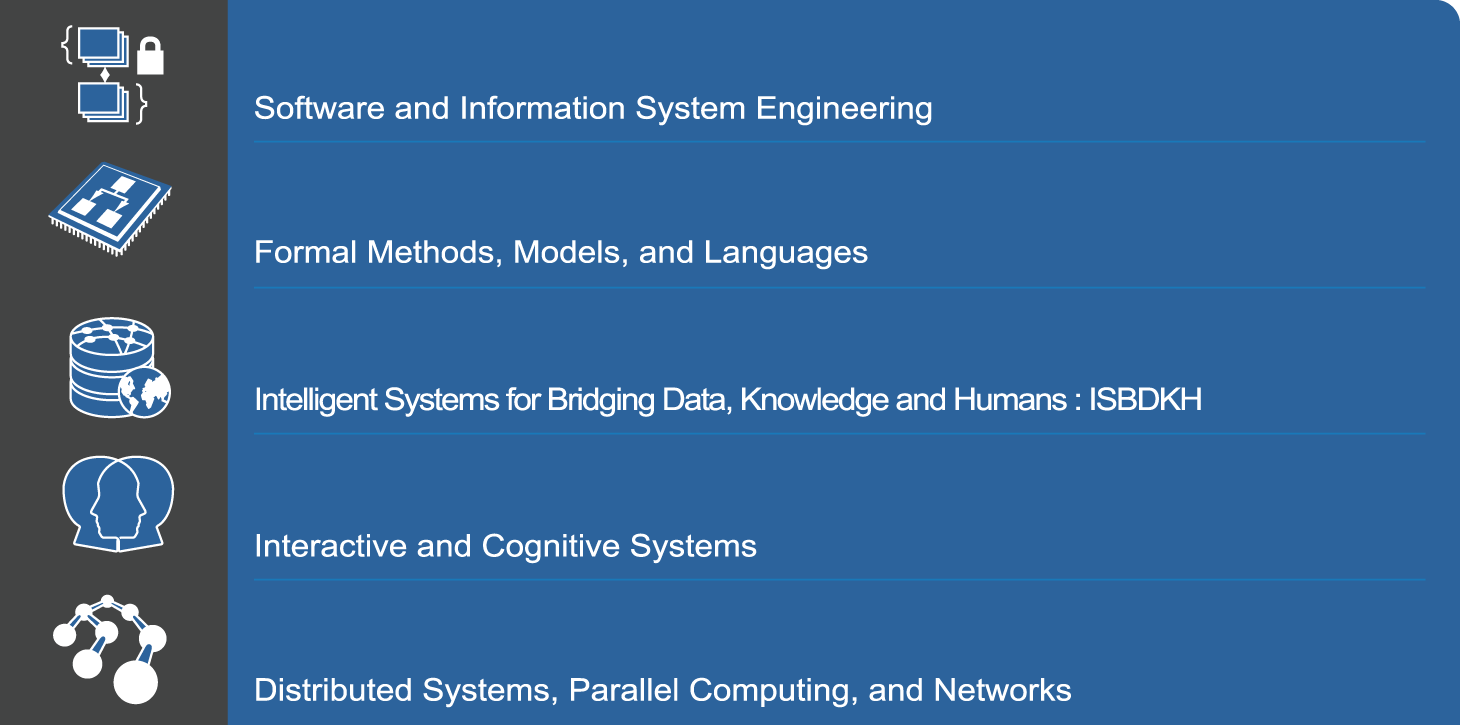
\includegraphics[width=12.5cm]{images/axeslig}
    \caption{Les différents axes de recherche du LIG.}
    \label{fig:lig}
\end{figure}

\subsection{Environement de travail}

Mon employeur officiel reste donc l'université, c'est-à-dire l'UGA. Mon équipe 
et moi-même étions localisé sur le campus, plus précisément dans le bâtiment 
``IMAG'', au quatrième étage consacré à la recherche dans le domaine 
informatique (voir mon bureau sur la Figure~\ref{fig:imag}).

\begin{figure}[h!t] \centering
    \begin{tabular}{@{}c@{\hspace{5pt}}c@{}}
    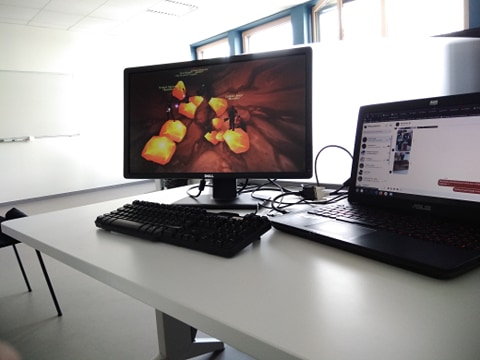
\includegraphics[width=0.49\textwidth]{images/desk} & 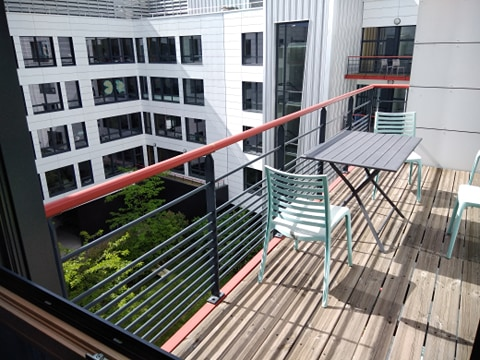
\includegraphics[width=0.49\textwidth]{images/balcony}
    \end{tabular}
    \caption{Bureau de travail et balcon vu de la fenêtre.}
    \label{fig:imag}
\end{figure}
